\subsection{命题 1：单期报告病例的精确分布与 Fisher 信息}

\subsubsection{原式与参数含义}

命题 1 讨论目标 A，即在给定当期共享环境的条件下测量当期传播参数 $R_t$。它建立在第~\ref{sec:model} 节的负二项分支与二项报告模型之上，并要求真实风险集规模 $n$ 与报告率 $\rho$ 已知。命题 1 第 (i) 条断言报告病例数在给定 $(n,R_t)$ 下仍服从负二项分布，原式如下：
\begin{equation*}
C_t \mid n, R_t \sim \operatorname{NB}\!\left(\text{均值} = \rho n R_t, \; \text{形状参数} = nk\right);
\tag{原文式 4}
\end{equation*}
命题 1 第 (iii) 条给出内部参数点上单期观测关于 $R_t$ 的 Fisher 信息，原式如下：
\begin{equation*}
\mathcal{I}(R_t \mid n) = \frac{n}{\frac{R_t}{\rho} + \frac{R_t^2}{k}};
\tag{原文式 5}
\end{equation*}
命题 1 第 (iv) 条断言矩估计量的条件方差恰好等于 Cramér--Rao 下界（下文简称 CRLB），原式如下：
\begin{equation*}
\operatorname{Var}\!\left(\frac{C_t}{\rho n} \;\middle|\; n, R_t\right) = \mathcal{I}(R_t \mid n)^{-1} = \frac{R_t}{\rho n} + \frac{R_t^2}{k n}.
\tag{原文式 6}
\end{equation*}

三个原式中出现的量含义如下。
\begin{itemize}
\item $C_t$ 是第 $t$ 期的报告病例数，取非负整数，是唯一的观测量。
\item $n$ 是上一代真实风险集规模，即产生第 $t$ 期继发感染的真实感染者人数，取正整数，在命题 1 中视为已知常数。
\item $R_t$ 是当期传播参数，即给定当期共享环境时每名感染者的期望继发感染数，取值于 $(0,\infty)$，是命题 1 的待估参数。
\item $\rho$ 是报告率，即每名真实感染者被独立报告的概率，取值于 $(0,1]$，假定已知且在期内不变。
\item $k$ 是个体继发感染数的负二项离散参数（Gamma 形状参数），取值于 $(0,\infty)$；$k$ 越小，少数个体贡献的继发感染越多，超传播越强 \citep{lloydsmith2005superspreading}，$k\to\infty$ 时个体继发感染数退化为 Poisson 分布。命题 1 的精确结论要求 $k$ 已知。
\item $nk$ 是 $C_t$ 的负二项形状参数，$\rho nR_t$ 是 $C_t$ 的条件期望，$\mathcal{I}(R_t\mid n)$ 是单期观测关于 $R_t$ 的 Fisher 信息。
\item $\widehat{R}_t=C_t/(\rho n)$ 是矩估计量，等于观测报告数除以单位 $R_t$ 对应的期望报告数 $\rho n$。
\end{itemize}

论文第 91 行只写出个体继发感染数 $X_{i,t}$ 的前两阶矩（原文式 1），附录第 688 行才使用完整分布。命题 1 的精确分布、极大似然与 CRLB 结论实际依赖下列四条假设。(a) 给定 $R_t$，$X_{1,t},\dots,X_{n,t}$ 独立同分布于 $\mathrm{NB}(k,p)$，$p=k/(k+R_t)$。(b) 同期 $n$ 名感染者共享同一个 $R_t$。(c) 给定真实感染数 $I_t=\sum_{i=1}^n X_{i,t}$，每名感染者独立地以概率 $\rho$ 被报告。(d) $k$ 与 $\rho$ 对推断者已知。下文推导逐条点明用到哪一条。

\subsubsection{逐步推导}

推导分六段完成，依次处理分布、矩、似然与极大似然估计、Fisher 信息、CRLB 取等与 UMVUE，以及 Poisson 极限。分布这一段只写结论和关键一步，完整证明见附录引理~\ref{lem:ap-nb} 与引理~\ref{lem:ap-thin}。
\begin{enumerate}
\item 由附录引理~\ref{lem:ap-nb}，个体继发感染数可写成 Poisson--Gamma 混合，其边缘分布为 $\mathrm{NB}(k,p)$，$p=k/(k+R_t)$，概率生成函数为 $G_X(s)=\bigl(p/(1-(1-p)s)\bigr)^{k}$。
\item 由独立随机变量之和的概率生成函数等于各自概率生成函数之积，并利用假设 (a)(b) 保证的“所有个体共用同一个 $p$”，得到 $G_{I_t}(s)=\bigl(p/(1-(1-p)s)\bigr)^{nk}$，即 $I_t\mid n,R_t\sim\mathrm{NB}(nk,p)$；若各人的 $R$ 不同，$p$ 不同，形状参数就不能简单相加。
\item 由附录引理~\ref{lem:ap-thin} 的抽稀复合关系 $G_{C_t}(s)=G_{I_t}(1-\rho+\rho s)$（依据假设 (c)），把自变量 $s$ 换成 $1-\rho+\rho s$；关键一步是把分母展开为 $1-(1-p)(1-\rho+\rho s)=[p+\rho(1-p)]-\rho(1-p)s$，分子分母同除以 $p+\rho(1-p)$ 后得到 $G_{C_t}(s)=\bigl(p^*/(1-(1-p^*)s)\bigr)^{nk}$。
\item 由代数化简，代入 $p=k/(k+R_t)$ 可得 $p+\rho(1-p)=(k+\rho R_t)/(k+R_t)$，于是 $p^*=k/(k+\rho R_t)$，$1-p^*=\rho R_t/(k+\rho R_t)$；由概率生成函数唯一决定分布，$C_t\mid n,R_t\sim\mathrm{NB}(nk,p^*)$，其概率质量函数为
\begin{equation*}
\Pr(C_t=c\mid n,R_t)=\frac{\Gamma(c+nk)}{c!\,\Gamma(nk)}\Bigl(\frac{k}{k+\rho R_t}\Bigr)^{nk}\Bigl(\frac{\rho R_t}{k+\rho R_t}\Bigr)^{c},\qquad c=0,1,2,\dots
\end{equation*}
\item 由负二项分布 $\mathrm{NB}(r,q)$ 的期望公式 $r(1-q)/q$ 与方差公式 $r(1-q)/q^2$，取 $r=nk$、$q=p^*$，可得
\begin{align*}
\mathbb{E}[C_t\mid n,R_t]&=nk\cdot\frac{\rho R_t}{k+\rho R_t}\cdot\frac{k+\rho R_t}{k}=\rho nR_t,\\
\operatorname{Var}(C_t\mid n,R_t)&=nk\cdot\frac{\rho R_t}{k+\rho R_t}\cdot\frac{(k+\rho R_t)^2}{k^2}=\frac{\rho nR_t(k+\rho R_t)}{k}=\rho nR_t+\frac{\rho^2nR_t^2}{k},
\end{align*}
原文式 4 中“均值 $=\rho nR_t$”即来自第一行。
\item 用全方差公式（附录引理~\ref{lem:ap-totvar}）以 $I_t$ 为条件变量复核方差：二项分布给出 $\mathbb{E}[\operatorname{Var}(C_t\mid I_t)]=\rho(1-\rho)\,\mathbb{E}[I_t]=\rho(1-\rho)nR_t$，第 2 步的负二项分布给出 $\operatorname{Var}(\mathbb{E}[C_t\mid I_t])=\rho^2\operatorname{Var}(I_t)=\rho^2(nR_t+nR_t^2/k)$，两项相加时 $\rho(1-\rho)nR_t+\rho^2nR_t=\rho nR_t$，结果与第 5 步一致。
\item 把第 5 步的方差除以期望的平方，得到报告病例数的相对方差
\begin{equation}
\frac{\operatorname{Var}(C_t\mid n,R_t)}{\mathbb{E}[C_t\mid n,R_t]^2}=\frac{1}{\rho nR_t}+\frac{1}{nk},
\label{eq:pa-relvar}
\end{equation}
它的第一项随期望报告数 $\rho nR_t$ 下降，第二项只与真实感染者数 $n$ 有关，后文命题 3 的非对称性即由式~(\ref{eq:pa-relvar}) 的第二项而来。
\item 对第 4 步的概率质量函数取对数，并把与 $R_t$ 无关的项 $\ln\Gamma(C_t+nk)-\ln C_t!-\ln\Gamma(nk)+nk\ln k+C_t\ln\rho$ 并入常数，得到对数似然
\begin{equation}
\ln L(R_t)=\text{const}-nk\ln(k+\rho R_t)+C_t\ln R_t-C_t\ln(k+\rho R_t)=\text{const}-(nk+C_t)\ln(k+\rho R_t)+C_t\ln R_t,
\label{eq:pa-loglik}
\end{equation}
与附录第 697 行的写法一致。
\item 对式~(\ref{eq:pa-loglik}) 关于 $R_t$ 求导，利用链式法则 $\frac{\mathrm d}{\mathrm dR_t}\ln(k+\rho R_t)=\rho/(k+\rho R_t)$，再通分并化简分子 $C_t(k+\rho R_t)-\rho R_t(nk+C_t)=C_tk+\rho R_tC_t-\rho nkR_t-\rho R_tC_t=k(C_t-\rho nR_t)$，得到得分函数
\begin{equation}
S(R_t)=\frac{\partial\ln L}{\partial R_t}=-\frac{\rho(nk+C_t)}{k+\rho R_t}+\frac{C_t}{R_t}=\frac{k(C_t-\rho nR_t)}{R_t(k+\rho R_t)}.
\label{eq:pa-score}
\end{equation}
\item 由式~(\ref{eq:pa-score}) 的符号分析判断最大值：当 $C_t>0$ 时分母 $R_t(k+\rho R_t)$ 恒正，得分在 $R_t<C_t/(\rho n)$ 时为正、在 $R_t>C_t/(\rho n)$ 时为负，所以 $\widehat{R}_t=C_t/(\rho n)$ 是 $(0,\infty)$ 上唯一的全局最大点，矩估计量与极大似然估计量（MLE）重合。
\item 由同一式在 $C_t=0$ 时的形式 $\ln L=\text{const}-nk\ln(k+\rho R_t)$ 可知似然关于 $R_t$ 严格递减，在开区间 $(0,\infty)$ 内没有最大点，在闭参数空间 $[0,\infty)$ 上于边界 $R_t=0$ 取最大值，这就是命题 1 第 (ii) 条的边界说明；下面关于 Fisher 信息和 CRLB 的陈述都限定在内部点 $R_t\in(0,\infty)$。
\item 由第 5 步的 $\mathbb{E}[C_t\mid n,R_t]=\rho nR_t$ 与期望的线性性，得到 $\mathbb{E}[\widehat{R}_t\mid n,R_t]=R_t$，即 $\widehat{R}_t$ 无偏；把同一结果代入式~(\ref{eq:pa-score}) 得 $\mathbb{E}[S(R_t)]=0$。
\item 由 Fisher 信息等于得分方差的定义，并利用得分是 $C_t$ 的线性函数、系数为 $k/[R_t(k+\rho R_t)]$，可得
\begin{equation*}
\mathcal{I}(R_t\mid n)=\frac{k^2\operatorname{Var}(C_t\mid n,R_t)}{R_t^2(k+\rho R_t)^2}=\frac{k^2\cdot\rho nR_t(k+\rho R_t)/k}{R_t^2(k+\rho R_t)^2}=\frac{k\rho n}{R_t(k+\rho R_t)}.
\end{equation*}
\item 把上式分子分母同除以 $k\rho$，分母变为 $R_t(k+\rho R_t)/(k\rho)=R_t/\rho+R_t^2/k$，于是 $\mathcal{I}(R_t\mid n)=n/(R_t/\rho+R_t^2/k)$，即原文式 5。
\item 由 Fisher 信息的第二种等价定义 $\mathcal{I}=-\mathbb{E}[\partial^2\ln L/\partial R_t^2]$（负二项支撑集 $\{0,1,2,\dots\}$ 与 $R_t$ 无关，求和与求导可交换，正则条件成立），先对式~(\ref{eq:pa-score}) 再求一次导，得到
\begin{equation*}
\frac{\partial^2\ln L}{\partial R_t^2}=-\frac{C_t}{R_t^2}+\frac{\rho^2(nk+C_t)}{(k+\rho R_t)^2}.
\end{equation*}
\item 对上式取期望并代入 $\mathbb{E}[C_t]=\rho nR_t$，利用 $nk+\rho nR_t=n(k+\rho R_t)$ 约去一个因子后通分，得到
\begin{equation*}
-\mathbb{E}\Bigl[\frac{\partial^2\ln L}{\partial R_t^2}\Bigr]=\frac{\rho n}{R_t}-\frac{\rho^2n}{k+\rho R_t}=\frac{\rho n[(k+\rho R_t)-\rho R_t]}{R_t(k+\rho R_t)}=\frac{k\rho n}{R_t(k+\rho R_t)},
\end{equation*}
与第 13 步完全一致，两种算法互证。
\item 把第 5 步的方差除以 $(\rho n)^2$，得到 $\operatorname{Var}(\widehat{R}_t\mid n,R_t)=(\rho nR_t+\rho^2nR_t^2/k)/(\rho^2n^2)=R_t/(\rho n)+R_t^2/(kn)$；而由第 14 步，$\mathcal{I}^{-1}=(R_t/\rho+R_t^2/k)/n$，两者逐项相等，这就是原文式 6。
\item 由 CRLB 的标准证明 \citep{casella2002statistical,lehmann1998point}，对任一无偏估计量 $T$，在 $\mathbb{E}[T]=R_t$ 两边对 $R_t$ 求导（支撑集不依赖参数，可交换求和与求导）得 $\operatorname{Cov}(T,S)=1$，再由 Cauchy--Schwarz 不等式 $\operatorname{Cov}(T,S)^2\le\operatorname{Var}(T)\operatorname{Var}(S)$ 得 $\operatorname{Var}(T)\ge1/\mathcal{I}(R_t\mid n)$。
\item 由 Cauchy--Schwarz 不等式的取等条件，上式取等当且仅当得分几乎处处是 $T$ 的仿射函数，即 $S(R_t)=\mathcal{I}(R_t)(T-R_t)$。对 $T=\widehat{R}_t$ 直接验算的结果如下式所示：
\begin{equation*}
\mathcal{I}(R_t\mid n)\Bigl(\frac{C_t}{\rho n}-R_t\Bigr)=\frac{k\rho n}{R_t(k+\rho R_t)}\cdot\frac{C_t-\rho nR_t}{\rho n}=\frac{k(C_t-\rho nR_t)}{R_t(k+\rho R_t)},
\end{equation*}
右端正是式~(\ref{eq:pa-score})。这一等式对每个正整数 $n$ 都成立，所以 CRLB 在每个有限样本上精确达到，与渐近理论无关。
\item 由指数族的标准写法，把第 4 步的概率质量函数改写成 $h(c)\exp\{\eta c-\psi(\eta)\}$，其中 $h(c)=\Gamma(c+nk)/(c!\,\Gamma(nk))$，自然参数 $\eta=\ln(1-p^*)=\ln\bigl(\rho R_t/(k+\rho R_t)\bigr)$，对数配分函数 $\psi(\eta)=-nk\ln(1-e^{\eta})$；验算时用到 $(1-p^*)^c=e^{\eta c}$ 与 $(p^*)^{nk}=(1-e^{\eta})^{nk}$。
\item 由自然参数的单调性，$\eta$ 关于 $R_t$ 严格递增，$R_t$ 取遍 $(0,\infty)$ 时 $\eta$ 取遍 $(-\infty,0)$，参数空间含开区间；由满秩指数族充分统计量的完备性定理 \citep{casella2002statistical}，$C_t$ 是 $R_t$ 的完备充分统计量。
\item 由 Lehmann--Scheffé 定理 \citep{lehmann1998point}，$\widehat{R}_t=C_t/(\rho n)$ 是完备充分统计量的函数且无偏，因此是 $R_t$ 唯一的一致最小方差无偏估计（UMVUE）。这条论证不需要 CRLB 的正则条件，但与第 18 步一样要求 $k$、$\rho$、$n$ 已知；若以估计值 $\hat k$ 代入，第 20 步的指数族结构不再对应固定的已知族，上述精确性质不再成立。
\item 由 $1/p^*=1+\rho R_t/k$ 把第 3 步的概率生成函数改写为 $G_{C_t}(s)=\bigl(1+\rho R_t(1-s)/k\bigr)^{-nk}=\bigl(1+\rho nR_t(1-s)/(nk)\bigr)^{-nk}$。
\item 由极限 $(1+x/N)^{N}\to e^{x}$（取 $N=nk\to\infty$），$k\to\infty$ 时 $G_{C_t}(s)\to\exp\{-\rho nR_t(1-s)\}$，这是 $\mathrm{Poisson}(\rho nR_t)$ 的概率生成函数；同时原文式 5 分母中的 $R_t^2/k\to0$，Fisher 信息趋于 $\rho n/R_t$。
\item 由 Poisson 均值参数 $\mu$ 的 Fisher 信息 $1/\mu$ 与重参数化公式 $\mathcal{I}(R_t)=(\partial\mu/\partial R_t)^2/\mu$，取 $\mu=\rho nR_t$ 得 $(\rho n)^2/(\rho nR_t)=\rho n/R_t$，与第 24 步的极限一致。
\end{enumerate}

论文在命题 1 之后给出的 Poisson 极限信息量如下式所示：
\begin{equation*}
\mathcal{I}(R_t \mid n) = \frac{\rho n}{R_t}
\tag*{原文第 151 行}
\end{equation*}
第 23--25 步说明它由两条路线得到同一结果，并与 Poisson 更新过程的信息标度律一致 \citep{parag2022quantifying}。

\subsubsection{直觉与数值例}

原文式 5 的分母 $R_t/\rho+R_t^2/k$ 是“每名真实感染者”贡献的方差，它由两部分相加：$R_t/\rho$ 来自 Poisson 计数与二项漏报，$R_t^2/k$ 来自个体传染力的离散。方差相加意味着信息按调和方式组合，任何一项变大都会压低每名感染者提供的信息 $1/(R_t/\rho+R_t^2/k)$。极大似然估计量与矩估计量重合的原因在于固定形状参数的负二项族是关于 $C_t$ 的单参数指数族，得分对 $C_t$ 是线性的，最优估计只能是 $C_t$ 的线性函数。

取论文图 1 参数 $\rho=0.25$、$k=0.35$，并令 $R_t=\bar R=1.15$。每名感染者的方差贡献为 $R_t/\rho=1.15/0.25=4.6$ 与 $R_t^2/k=1.3225/0.35=3.7786$，合计 $8.3786$，每名感染者的信息为 $1/8.3786=0.11935$。在 $n=10$（期望报告规模 $m=\rho n=2.5$）时，$\mathcal{I}=10\times0.11935=1.1935$，$\operatorname{Var}(\widehat{R}_t)=0.46+0.37786=0.83786$，变异系数为 $\sqrt{0.83786}/1.15=0.9153/1.15=0.796$；其中超传播项占 $3.7786/8.3786=45.1\%$。若 $k\to\infty$，Poisson 极限信息为 $\rho n/R_t=2.5/1.15=2.1739$，有限 $k$ 使信息损失同样的 $45.1\%$。在 $n=40$（$m=10$）时，$\operatorname{Var}(\widehat{R}_t)=1.15/10+1.3225/14=0.115+0.09446=0.20946$，这就是原文图 1(a) 蓝线在 $m=10$ 处的值。

\subsubsection{与仿真和实证的对应}

原文图 1(a) 的蓝线画出原文式 6 随 $m=\rho n$ 的双对数曲线，斜率为 $-1$ 并趋于零；原文图 1(b) 报告仿真方差与理论方差之比在全部参数网格上处于 0.988--1.017（原文第 196 行），仿真为 50,000 次独立重复（原文第 419 行）。我们的独立核验分三层。符号层面，抽稀后的概率生成函数、$p^*$、两阶矩、对数似然、得分、MLE、两种 Fisher 信息算法、CRLB、得分的仿射条件与 Poisson 极限共 13 项全部用符号计算核对成立。数值层面，对三组参数逐点卷积再抽稀得到的分布与 $\mathrm{NB}(nk,p^*)$ 的总变差距离不超过 $5.24\times10^{-15}$，处于浮点误差量级。蒙特卡洛层面的结果列于表~\ref{tab:pa-mc1}：三组配置下估计量方差与原文式 6 的比值为 0.9830--1.0199，$|z|\le1.35$，得分方差与原文式 5 的比值为 0.9828--1.0198，卡方拟合的 $p$ 值均高于预设门槛 0.001。

\begin{table}[!tbp]
\centering
\small
\caption{命题 1 的蒙特卡洛核验：估计量方差、得分方差与分布拟合（三组参数配置）}
\label{tab:pa-mc1}
\begin{tabular}{L{3.2cm}L{1.3cm}L{1.4cm}L{1.4cm}L{1.1cm}L{0.9cm}L{1.5cm}L{1.5cm}}
\toprule
配置 $(n,k,\rho,R_t)$ & 重复次数 & 理论方差 & 模拟方差 & 比值 & $z$ & 得分方差比 & 卡方 $p$ 值 \\
\midrule
$(10,\,0.35,\,0.25,\,1.15)$ & 20000 & 0.83786 & 0.85449 & 1.0199 & 1.35 & 1.0198 & 0.011 \\
$(20,\,0.1,\,0.5,\,1.5)$ & 10000 & 1.27500 & 1.27996 & 1.0039 & 0.17 & 1.0038 & 0.466 \\
$(40,\,2.0,\,0.8,\,0.8)$ & 5000 & 0.03300 & 0.03244 & 0.9830 & $-0.85$ & 0.9828 & 0.861 \\
\bottomrule
\end{tabular}
\end{table}

实证部分不直接检验命题 1，因为目标 A 的真值 $R_t$ 在住院数据中不可观测；命题 1 在全文中的作用是为命题 2 提供内层条件方差（见第~\ref{sec:empirical} 节对实证映射的讨论）。

\subsubsection{原文表述的问题}

第一，原文第 196 行称图 1(b) 验证了“有限样本下 Cramér--Rao 下界的代数紧致性”，第 419 行称仿真“严格确认了 Cramér--Rao 下界的有限样本收敛性”。由第 19 步，CRLB 在每个有限 $n$ 上精确达到，没有任何收敛过程；图 1(b) 中 0.988--1.017 的偏离来自蒙特卡洛误差。以正态近似估算，50,000 次重复下样本方差的相对标准误约为 $\sqrt{2/50000}=0.0063$；负二项分布的超额峰度使实际标准误更大，表~\ref{tab:pa-mc1} 第一行由比值与 $z$ 值反推的相对标准误约为 $0.0199/1.35=0.015$（20,000 次重复）。建议把第 419 行改为“仿真方差与理论值之比处于 0.988--1.017，偏离在蒙特卡洛误差范围内，与 CRLB 精确达到一致”。

第二，附录第 715 行由“严格达到 CRLB”直接断言估计量为一致最小方差无偏估计，缺少论证。正则条件下的 CRLB 论证（第 18--19 步）与 Lehmann--Scheffé 论证（第 20--22 步）都可以补上，后者更干净，建议在附录补一句：“固定 $nk$ 时 $\{\mathrm{NB}(nk,p^*(R_t))\}$ 为关于 $C_t$ 的单参数指数族，$C_t$ 完备充分，由 Lehmann--Scheffé 定理，$C_t/(\rho n)$ 为 UMVUE。”

第三，原文式 1 只给出两阶矩，而命题 1 的“严格服从负二项分布”需要完整分布假设 (a) 与同期共享环境假设 (b)。两者以及“$k$、$\rho$ 已知”应在第 94 行之后集中写成一条假设。答辩时被问到“$k$ 用估计值时结论是否仍精确”可直接回答：不再精确，只在大样本下近似成立。

\subsection{命题 2：跨期基础水平的单期方差}

\subsubsection{原式与参数含义}

命题 2 把推断目标从当期参数 $R_t$ 换成跨期基础水平 $\bar R$（目标 B），估计量仍是单期的 $C_t/(\rho n)$。命题 2 给出的单期估计量对 $\bar R$ 的条件边际方差如下式所示：
\begin{equation*}
\operatorname{Var}\!\left(\frac{C_t}{\rho n} \;\middle|\; n\right) = v_R + \frac{\bar{R}}{\rho n} + \frac{\bar{R}^2 + v_R}{k n}.
\tag{原文式 7}
\end{equation*}
论文第 174 行令 $m=\rho n$，把原文式 7 改写成 $v_R+A/m$，其中规模相关方差系数 $A$ 的定义如下：
\begin{equation*}
A = \bar{R} + \frac{\rho(\bar{R}^2 + v_R)}{k}.
\tag{原文式 8}
\end{equation*}

两式中新出现的量含义如下，$n$、$\rho$、$k$ 的含义同命题 1。
\begin{itemize}
\item $\bar R=\mathbb{E}[R_t\mid n]$ 是跨期基础水平，取值于 $(0,\infty)$，论文图 1 取 $1.15$。
\item $v_R=\operatorname{Var}(R_t\mid n)$ 是不可约环境方差，即当期共享环境造成的 $R_t$ 跨期波动，取正值，论文图 1 取 $0.04$。
\item $m=\rho n$ 是上一代真实风险集对应的期望被报告人数，单位为例每期；论文第 174 行特意说明，它与当期报告数的条件期望 $\rho nR_t$ 不同，后者的期望为 $\bar R m$。
\item $A$ 是规模相关方差系数，取正值，图 1 参数下为 $2.12321$；它显式依赖报告率 $\rho$（原文第 187 行），所以两个 $m$ 相同而 $\rho$ 不同的系统具有不同的 $A$。
\end{itemize}

命题 2 用到原文式 3 的条件矩假设 $\mathbb{E}[R_t\mid n]=\bar R$、$\operatorname{Var}(R_t\mid n)=v_R$，以及命题 1 的两个结论（条件无偏与条件方差）。它还隐含要求同期 $n$ 名感染者共享同一个 $R_t$，这一点在下文的直觉部分专门说明。

\subsubsection{逐步推导}

\begin{enumerate}
\item 由全方差公式（附录引理~\ref{lem:ap-totvar}），在给定 $n$ 的条件下以 $R_t$ 为条件变量分解：
\begin{equation}
\operatorname{Var}\Bigl(\frac{C_t}{\rho n}\Bigm| n\Bigr)=\operatorname{Var}\Bigl(\mathbb{E}\Bigl[\frac{C_t}{\rho n}\Bigm| n,R_t\Bigr]\Bigm| n\Bigr)+\mathbb{E}\Bigl[\operatorname{Var}\Bigl(\frac{C_t}{\rho n}\Bigm| n,R_t\Bigr)\Bigm| n\Bigr].
\label{eq:pa-totvar}
\end{equation}
\item 由命题 1 第 12 步的条件无偏性 $\mathbb{E}[C_t/(\rho n)\mid n,R_t]=R_t$，式~(\ref{eq:pa-totvar}) 的第一项等于 $\operatorname{Var}(R_t\mid n)$，再由原文式 3 得到 $v_R$。
\item 由原文式 6，内层条件方差为 $R_t/(\rho n)+R_t^2/(kn)$，它是 $R_t$ 的二次函数，外层期望要对 $R_t$ 的一次项与二次项分别计算。
\item 由条件期望的线性性，式~(\ref{eq:pa-totvar}) 的第二项等于 $\mathbb{E}[R_t\mid n]/(\rho n)+\mathbb{E}[R_t^2\mid n]/(kn)$，其中第一部分由原文式 3 直接得到 $\bar R/(\rho n)$。
\item 由方差的定义 $\operatorname{Var}(R_t\mid n)=\mathbb{E}[R_t^2\mid n]-\mathbb{E}[R_t\mid n]^2$ 移项，得到二阶矩 $\mathbb{E}[R_t^2\mid n]=\bar R^2+v_R$（附录第 728 行），因此第二部分为 $(\bar R^2+v_R)/(kn)$。分子中的 $v_R$ 最容易被漏掉：超传播方差 $R_t^2/k$ 是 $R_t$ 的凸函数，由 Jensen 不等式 $\mathbb{E}[R_t^2]\ge(\mathbb{E}R_t)^2$，环境波动会抬高平均的超传播噪声，抬高的量恰为 $v_R/(kn)$。
\item 把第 2、4、5 步的三项相加，得到 $v_R+\bar R/(\rho n)+(\bar R^2+v_R)/(kn)$，即原文式 7。
\item 由 $m=\rho n$ 推出 $1/n=\rho/m$，代入后两项得 $\bar R/(\rho n)=\bar R/m$ 与 $(\bar R^2+v_R)/(kn)=\rho(\bar R^2+v_R)/(km)$，提出公因子 $1/m$ 得
\begin{equation*}
\frac{\bar R}{\rho n}+\frac{\bar R^2+v_R}{kn}=\frac{1}{m}\Bigl[\bar R+\frac{\rho(\bar R^2+v_R)}{k}\Bigr]=\frac{A}{m},
\end{equation*}
所以原文式 7 可写成 $V(m)=v_R+A/m$，方括号内即原文式 8。
\end{enumerate}

\subsubsection{直觉与数值例}

单期观测无论数得多准，测到的也只是一期环境的实现 $R_t$，而 $R_t$ 围绕 $\bar R$ 的波动 $v_R$ 只有多观测几期（命题 4）或在环境不完全相关的多个地区汇总才能平均掉。$v_R$ 不随 $n$ 下降，根源在于同期共享环境的假设 (b)。作为对照，假设每名感染者各自独立抽取一个 $R_i$（期望 $\bar R$、方差 $v_R$），由全方差公式先得单人方差，再由独立性与二项抽稀得
\begin{align*}
\operatorname{Var}(X_i)&=\mathbb{E}\Bigl[R_i+\frac{R_i^2}{k}\Bigr]+\operatorname{Var}(R_i)=\bar R+\frac{\bar R^2+v_R}{k}+v_R,\\
\operatorname{Var}\Bigl(\frac{C_t}{\rho n}\Bigr)&=\frac{\rho(1-\rho)n\bar R+\rho^2n\operatorname{Var}(X_i)}{\rho^2n^2}=\frac{\bar R}{\rho n}+\frac{\bar R^2+v_R}{kn}+\frac{v_R}{n},
\end{align*}
此时环境项被稀释为 $v_R/n$，不可约下限消失。命题 2 的“环境下限”因此是共享环境假设的直接产物，这与种群动态中人口统计随机性随规模平均、环境随机性不随规模平均的区分相对应 \citep{engen1998demographic}。

取论文图 1 参数 $\bar R=1.15$、$v_R=0.04$、$k=0.35$、$\rho=0.25$。先算 $A$：$\bar R^2+v_R=1.3225+0.04=1.3625$，$\rho(\bar R^2+v_R)/k=0.340625/0.35=0.97321$，故 $A=1.15+0.97321=2.12321$。在 $n=40$（$m=10$）时三项分别为 $v_R=0.04$、$\bar R/(\rho n)=1.15/10=0.115$、$(\bar R^2+v_R)/(kn)=1.3625/14=0.09732$，合计 $0.25232$，与 $v_R+A/m=0.04+0.21232$ 相同；其中由第 5 步额外引入的 $v_R/(kn)=0.04/14=0.00286$ 只占 2.9\% 的超传播项，数值上小，概念上不能省。与命题 1 在 $R_t=\bar R$ 处的 $0.20946$ 相比，目标 B 的方差多出 $0.04286=v_R+v_R/(kn)$。在 $n=2000$（$m=500$）时 $V=0.04+0.00425=0.04425$，环境项已占 $90.4\%$。

\subsubsection{与仿真和实证的对应}

原文图 1(a) 的红线是原文式 7，随 $m$ 增大平稳趋于环境下限 $v_R=0.04$（原文第 196 行）。我们的符号核验确认全方差分解给出原文式 7、且原文式 7 等于 $v_R+A/m$；蒙特卡洛核验在四个规模上比较了理论方差与模拟方差，结果见表~\ref{tab:pa-mc2}，比值处于 0.9867--1.0082，$|z|\le2.44$，均在预设容差内。

\begin{table}[!tbp]
\centering
\small
\caption{命题 2 的理论方差 $v_R+A/m$ 与蒙特卡洛模拟值（论文图 1 参数）}
\label{tab:pa-mc2}
\begin{tabular}{L{1.2cm}L{1.2cm}L{2.0cm}L{2.0cm}L{1.6cm}L{1.2cm}L{2.6cm}}
\toprule
$n$ & $m$ & 理论方差 & 模拟方差 & 比值 & $z$ & 环境项份额（理论/模拟） \\
\midrule
4 & 1 & 2.16321 & 2.13452 & 0.9867 & $-2.25$ & 0.018 / 0.019 \\
40 & 10 & 0.25232 & 0.25216 & 0.9993 & $-0.17$ & 0.159 / 0.159 \\
212 & 53 & 0.08006 & 0.08045 & 1.0048 & 1.39 & 0.500 / 0.499 \\
2000 & 500 & 0.04425 & 0.04461 & 1.0082 & 2.44 & 0.904 / 0.904 \\
\bottomrule
\end{tabular}
\end{table}

原文图 3(a) 把 $V(m)=v_R+A/m$（$A=2.1232$，$v_R=0.04$）作为更新过程仿真的参照曲线（原文第 399 行）。更新过程中风险集由上一期传播生成，命题 2 的条件不再严格成立；原文第 393 行自己报告以初始参数为横轴时表观比值为 0.75--0.98 倍，所以 $V(m)$ 在该口径下不构成下界，详细讨论见第~\ref{sec:checks} 节。

实证部分用仿射关系“相对损失 $=a+b/D_t$”（原文式 31）映射命题 2：截距 $a$ 对应 $v_R/\bar R^2$，斜率 $b$ 对应 $A/\bar R^2$。命题 2 预言的“常数加 $1/D_t$”结构在住院数据中定性成立，但数量上不吻合：$a=0.0991$ 是情景隐含值 0.014--0.029 的 3.5--6.9 倍，$b=2.2434$ 是情景隐含值 0.610--0.707 的 3.2--3.7 倍，原因分析见第~\ref{sec:empirical} 节。

\subsubsection{原文表述的问题}

第一，原文第 168 行称 $v_R$ 是“无法随横截面聚合消除的不可约环境方差”，而第 617 行在全国汇总时恰好利用各州环境不完全相关来压低环境方差，论文给出的汇总后环境方差如下式所示：
\begin{equation*}
v_R^{\mathrm{agg}} = v_R \left[\bar{c} + \frac{1-\bar{c}}{J}\right]
\tag*{原文第 617 行}
\end{equation*}
其中 $J$ 是汇总的辖区数，$\bar c$ 是辖区间环境扰动的平均相关系数。$\bar c<1$ 时 $v_R^{\mathrm{agg}}<v_R$，与第 168 行的说法矛盾。由上面的对照推导，$v_R$ 只在所有单位共享同一个 $R_t$ 时不可约。建议第 168 行改为“无法通过同一环境内扩大规模消除；跨相关性不完全的环境聚合可削减其 $(1-\bar c)$ 部分（见第 617 行）”。

第二，原文式 3 的条件 $\mathbb{E}[R_t\mid n]=\bar R$ 对设计固定的 $n$ 成立（原文第 114 行给出的充分条件）。在时间序列中 $n_t=I_{t-1}$ 由 $R_{t-1}$ 生成，若环境存在自相关，$n_t$ 偏大意味着 $R_{t-1}$ 偏大，进而 $R_t$ 也偏大，这一条件不再自动成立。实证部分把病例规模当作外生规模时，应在局限性中说明这一点。

\subsection{定义 1：方差占比交叉点 $m_\times$}

\subsubsection{原式与参数含义}

定义 1 把命题 2 的两项方差相等处的规模命名为交叉点，原文的定义式如下：
\begin{equation*}
m_\times \triangleq \frac{A}{v_R} = \frac{\bar{R} + \rho(\bar{R}^2 + v_R)/k}{v_R}.
\tag{原文式 9}
\end{equation*}
论文在“经济学与监测含义”一段给出总方差对规模的导数，用来说明 $m_\times$ 处不存在突变：
\begin{equation*}
\frac{\mathrm{d}V}{\mathrm{d}m} = -\frac{A}{m^2}
\tag*{原文第 190 行}
\end{equation*}
论文在更新过程仿真一节给出规模翻倍带来的相对方差降幅，用来量化越过交叉点后收益的衰减：
\begin{equation*}
\frac{V(m) - V(2m)}{V(m)} = \frac{1}{2(1 + m/m_\times)}.
\tag{原文式 29}
\end{equation*}

\begin{itemize}
\item $V(m)=v_R+A/m$ 是命题 2 的单期方差，看成 $m$ 的函数时固定 $\rho$、$k$、$\bar R$、$v_R$，即沿扩大 $n$ 的方向变化（原文第 190 行“沿扩大 $n$ 方向”）。
\item $m_\times$ 是方差占比交叉点，单位与 $m$ 相同（例每期），取正值，要求 $v_R>0$；图 1 参数下为 $53.08$。
\item $A$、$v_R$ 的含义同命题 2；因为 $A$ 依赖 $\rho$，$m_\times$ 也依赖 $\rho$，比较不同报告率的系统时 $m_\times$ 不是同一个数。
\end{itemize}

\subsubsection{逐步推导}

\begin{enumerate}
\item 由交叉点的定义令规模项等于环境项 $A/m=v_R$，解得 $m=A/v_R$；再把原文式 8 代入分子，就得到原文式 9 的第二种写法。
\item 由份额的定义，规模项在总方差中的份额为 $(A/m)/(v_R+A/m)$，分子分母同乘 $m/A$ 并利用 $v_R/A=1/m_\times$，得到
\begin{equation}
s(m)=\frac{A/m}{v_R+A/m}=\frac{1}{1+m/m_\times},\qquad 1-s(m)=\frac{m}{m+m_\times},
\label{eq:pa-share}
\end{equation}
其中 $1-s(m)$ 是环境项份额；在 $m=m_\times$ 处两者都等于 $1/2$，这就是原文“两项各占 50\%”的来源。
\item 由幂函数求导法则 $\frac{\mathrm d}{\mathrm dm}m^{-1}=-m^{-2}$，得到 $\mathrm dV/\mathrm dm=-A/m^2<0$，即原文第 190 行；$V$ 在 $(0,\infty)$ 上严格递减，在 $m_\times$ 处的斜率为 $-A/m_\times^2=-v_R/m_\times$。
\item 再求一次导得 $\mathrm d^2V/\mathrm dm^2=2A/m^3>0$，二阶导在整个 $(0,\infty)$ 上恒正、从不变号，所以 $V$ 严格凸且没有拐点；$m_\times$ 在 $V$ 曲线上不对应任何几何特殊点，它的意义要从份额与弹性来理解。
\item 由弹性的定义 $\varepsilon(m)=(\mathrm dV/\mathrm dm)\cdot(m/V)$，代入第 3 步并利用式~(\ref{eq:pa-share})，得到
\begin{equation}
\varepsilon(m)=\frac{-A/m}{v_R+A/m}=-\frac{1}{1+m/m_\times}=-\frac{m_\times}{m+m_\times}=-s(m),
\label{eq:pa-elastic}
\end{equation}
即弹性等于规模项份额的相反数；$m\ll m_\times$ 时 $\varepsilon\to-1$（规模加倍、方差近似减半），$m=m_\times$ 时 $\varepsilon=-1/2$，$m\gg m_\times$ 时 $\varepsilon\to0$。式~(\ref{eq:pa-elastic}) 也是双对数坐标下总方差曲线的斜率 $\mathrm d\ln V/\mathrm d\ln m$。
\item 由 $V(m)=v_R+A/m$ 直接相减，环境项抵消，得到翻倍的绝对降幅 $V(m)-V(2m)=A/m-A/(2m)=A/(2m)$。
\item 把第 6 步除以 $V(m)$ 并把分子分母同除以 $A$，利用 $v_R/A=1/m_\times$ 化简，得到
\begin{equation}
\frac{V(m)-V(2m)}{V(m)}=\frac{A/(2m)}{v_R+A/m}=\frac{A}{2(v_Rm+A)}=\frac{1}{2(1+m/m_\times)}=\frac{s(m)}{2},
\label{eq:pa-halving}
\end{equation}
前四个表达式即原文式 29；最后一个等号说明翻倍降幅是规模项份额的一半，上限 50\% 只在 $m\to0$ 时达到。
\end{enumerate}

\subsubsection{直觉与数值例}

规模项每翻一倍就砍掉自身的一半，但它在总方差中只占 $s(m)$，所以总降幅等于 $s(m)/2$（式~(\ref{eq:pa-halving})）。$m_\times$ 因此是一个刻度：规模低于它时，增加病例数主要压缩规模项，弹性接近 $-1$；规模高于它时，大部分方差来自环境，翻倍的收益迅速收窄，但始终为正。

代入论文图 1 参数，$m_\times=A/v_R=2.12321/0.04=53.08$。翻倍降幅的三个代表点为：$m=10$ 时 $m/m_\times=10/53.08=0.18839$，降幅 $1/(2\times1.18839)=42.07\%$，约为 42.1\%；$m=m_\times$ 时降幅 $1/(2\times2)=25.0\%$；$m=200$ 时 $m/m_\times=3.7679$，降幅 $1/(2\times4.7679)=10.49\%$，约为 10.5\%。表~\ref{tab:pa-share} 列出更多规模下的分解，图~\ref{fig:pa-variance} 把同一组数值画成曲线。

\begin{table}[!tbp]
\centering
\small
\caption{论文图 1 参数下单期方差 $V(m)=v_R+A/m$ 的分解、弹性与翻倍降幅（$A=2.12321$，$v_R=0.04$，$m_\times=53.08$）}
\label{tab:pa-share}
\begin{tabular}{L{1.4cm}L{1.8cm}L{1.8cm}L{2.0cm}L{2.0cm}L{1.6cm}L{2.0cm}}
\toprule
$m$ & $A/m$ & $V(m)$ & 规模项份额 & 环境项份额 & 弹性 & 翻倍降幅 \\
\midrule
1 & 2.12321 & 2.16321 & 98.2\% & 1.8\% & $-0.982$ & 49.08\% \\
10 & 0.21232 & 0.25232 & 84.1\% & 15.9\% & $-0.841$ & 42.07\% \\
25 & 0.08493 & 0.12493 & 68.0\% & 32.0\% & $-0.680$ & 33.99\% \\
53.08 & 0.04000 & 0.08000 & 50.0\% & 50.0\% & $-0.500$ & 25.00\% \\
100 & 0.02123 & 0.06123 & 34.7\% & 65.3\% & $-0.347$ & 17.34\% \\
200 & 0.01062 & 0.05062 & 21.0\% & 79.0\% & $-0.210$ & 10.49\% \\
500 & 0.00425 & 0.04425 & 9.6\% & 90.4\% & $-0.096$ & 4.80\% \\
\bottomrule
\end{tabular}
\end{table}

\begin{figure}[!tbp]
\centering
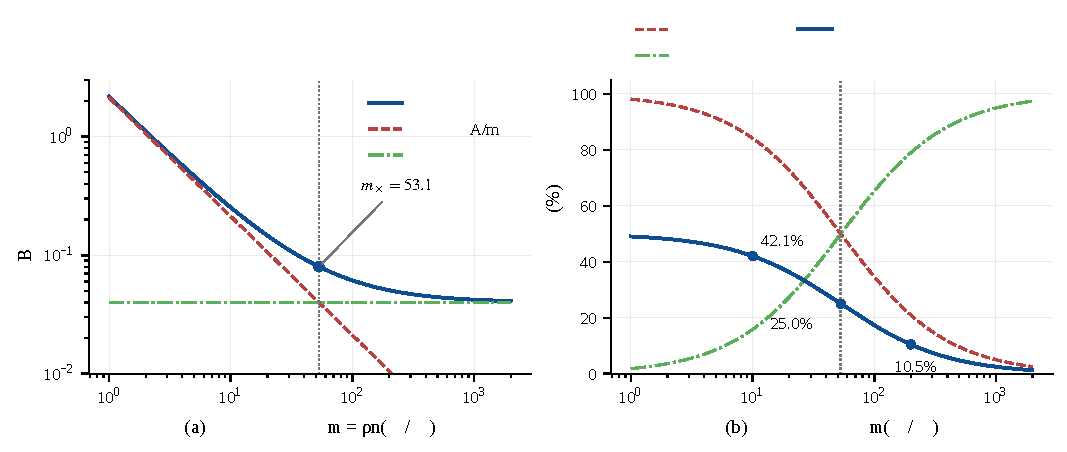
\includegraphics[width=0.95\linewidth]{figures/fig_variance_scale.pdf}
\caption{论文图 1 参数（$\bar R=1.15$，$v_R=0.04$，$k=0.35$，$\rho=0.25$）下目标 B 的单期方差随期望报告规模 $m=\rho n$ 的变化。左图在对数坐标下画出总方差 $v_R+A/m$、规模项 $A/m$ 与环境下限 $v_R$，二者在交叉点 $m_\times=53.1$ 相交，此处总方差为 $2v_R$。右图给出规模项占比、环境项占比以及规模翻倍带来的方差降幅，降幅在 $m=10$、$m_\times$、$m=200$ 处分别为 42.1\%、25.0\%、10.5\%，恒等于规模项占比的一半。}
\label{fig:pa-variance}
\end{figure}

图~\ref{fig:pa-variance} 左图中总方差曲线在小规模端贴着斜率 $-1$ 的规模项，在大规模端趋平于 $v_R$，中间平滑过渡，看不到任何折点，这正是第 4 步“严格凸、无拐点”的图形表现。右图中翻倍降幅曲线与规模项份额曲线处处相差一半，对应式~(\ref{eq:pa-halving})。

\subsubsection{与仿真和实证的对应}

原文图 1(c) 展示误差预算的演变，并标出在 $m_\times=53.1$ 处两项各占 50\%（原文第 196 行）。我们的核验确认 $A=2.1232$、$m_\times=53.08$，$m=m_\times$ 处环境项份额精确为 $1/2$，导数与翻倍降幅公式符号成立；表~\ref{tab:pa-mc2} 最后一列显示蒙特卡洛估计的环境项份额在 $m=1,10,53,500$ 处为 0.019、0.159、0.499、0.904，与理论值 0.018、0.159、0.500、0.904 一致。原文图 3(c) 与第 399、409 行报告的翻倍降幅 42.1\%、25.0\%、10.5\% 与精确值 42.07\%、25.00\%、10.49\% 一致；同一图中更新过程的经验降幅在 $m<12$ 段系统性高于解析式（$m=6\to12$ 为 73.5\%），这一偏离属于更新过程的额外误差，不影响定义 1 本身的代数。

实证部分用 $m_\times^{\mathrm{emp}}=b/a=2.2434/0.0991=22.6$ 与流感住院情景区间 21.3--49.3（原文第 515 行）比较。情景区间上端按一致参数应为 49.18。更关键的是，分母由报告病例构造时二项噪声会放大斜率：在原始滞后权重下，含噪分母使 $b/a$ 的期望由真实的 30.7 升到 59.2。实证中截距也被放大，两者部分抵消，所以“同一量级”不能当作 $m_\times$ 的结构性验证，详见第~\ref{sec:empirical} 节。

\subsubsection{原文表述的问题}

第一，原文第 187 行和图 1(c) 图注把 $m_\times$ 称为“收益拐点”。由第 4 步，$V$ 严格凸，没有拐点；$m_\times$ 是弹性等于 $-1/2$、两项份额各半的刻度。建议全文统一称“方差占比交叉点”，并在第 190 行补上弹性 $-m_\times/(m+m_\times)$，这比“导数平滑连续、不存在突变”更能说明交叉点的经济含义。

第二，原文图 1(c) 中交叉点的标注在 PDF 中渲染为“m imes”，是乘号命令的转义错误，应在作图脚本中修正。

\subsection{命题 3：扩大基数与提高报告率}

\subsubsection{原式与参数含义}

论文为比较两条增加报告病例的政策路径，把原文式 7 写成 $(n,\rho)$ 的二元函数，如下式所示：
\begin{equation*}
V(n, \rho) = v_R + \frac{\bar{R}}{\rho n} + \frac{\bar{R}^2 + v_R}{k n}.
\tag{原文式 10}
\end{equation*}
为分离报告率的作用，论文把第二项恒等拆分为完全报告时的计数项与漏报项，如下式所示：
\begin{equation*}
\frac{\bar{R}}{\rho n} = \frac{\bar{R}}{n} + \frac{(1-\rho)\bar{R}}{\rho n}.
\tag{原文式 11}
\end{equation*}
命题 3 第 (i) 条给出报告率趋于 1 时的饱和下界，原式如下：
\begin{equation*}
\lim_{\rho \to 1} V(n, \rho) = v_R + \frac{\bar{R}}{n} + \frac{\bar{R}^2 + v_R}{k n} > v_R.
\tag{原文式 12}
\end{equation*}
命题 3 第 (ii) 条给出风险集规模趋于无穷时的极限，原式如下：
\begin{equation*}
\lim_{n \to \infty} V(n, \rho) = v_R.
\tag{原文式 13}
\end{equation*}

\begin{itemize}
\item $n$ 是真实风险集规模，取正整数，求极限时把它看成可以连续增大的量；扩大 $n$ 对应扩大哨点覆盖或跨区域汇总感染者。
\item $\rho$ 是报告率，取值于 $(0,1]$；提高 $\rho$ 对应加强筛查、降低检测门槛。
\item $\bar R/n$ 是完全报告时仍存在的 Poisson 计数波动，$(1-\rho)\bar R/(\rho n)$ 是漏报额外引入的抽样方差，$(\bar R^2+v_R)/(kn)$ 是个体超传播造成的子代抽样方差。
\item $v_R$、$\bar R$、$k$ 的含义同命题 2，在命题 3 中都视为固定。
\end{itemize}

\subsubsection{逐步推导}

\begin{enumerate}
\item 由原文式 7 把 $n$ 与 $\rho$ 分开书写即得原文式 10，它在数值上就是命题 2 的方差，没有新增假设。
\item 由通分可验证原文式 11：右端为 $[\rho\bar R+(1-\rho)\bar R]/(\rho n)=\bar R/(\rho n)$。
\item 对原文式 10 关于 $\rho$ 求偏导，只有第二项含 $\rho$，得 $\partial V/\partial\rho=-\bar R/(\rho^2n)<0$；因此 $V$ 关于 $\rho$ 严格递减，而超传播项 $(\bar R^2+v_R)/(kn)$ 与 $\rho$ 无关，提高 $\rho$ 对它没有作用。
\item 由 $V$ 关于 $\rho$ 的连续性取 $\rho\to1$，漏报项 $(1-\rho)\bar R/(\rho n)\to0$，得到原文式 12 的等号部分；由于 $n<\infty$，$\bar R/n$ 与 $(\bar R^2+v_R)/(kn)$ 都严格为正，所以极限严格大于 $v_R$。结合第 3 步的单调性，这个极限值也是 $V$ 在 $\rho\in(0,1]$ 上的最小值，等于 $V(n,1)$。
\item 对原文式 10 关于 $n$ 求偏导得 $\partial V/\partial n=-[\bar R/\rho+(\bar R^2+v_R)/k]/n^2<0$；由 $1/n\to0$，后两项都是 $O(1/n)$，对任意固定的 $\rho\in(0,1]$ 都趋于零，得到原文式 13。
\item 由 $n=m/\rho$ 把原文式 10 改写为 $(m,\rho)$ 的函数
\begin{equation*}
V=v_R+\frac{\bar R}{m}+\frac{\rho(\bar R^2+v_R)}{km},
\end{equation*}
可见固定 $m$ 时提高 $\rho$ 等于缩小 $n$，超传播项反而变大；这就是原文第 187 行所说“$A$ 依赖 $\rho$”与命题 3 非对称性的同一来源。
\item 命题 3 只比较了极限，政策上更有用的是边际比较：让 $m$ 增加同样的比例，一次沿 $n$、一次沿 $\rho$。由对数求导 $\partial V/\partial\ln n=n\,\partial V/\partial n$，沿 $n$ 方向得 $\partial V/\partial\ln n=-\bar R/(\rho n)-(\bar R^2+v_R)/(kn)=-A/m$。
\item 同理沿 $\rho$ 方向只有第二项变化，得 $\partial V/\partial\ln\rho=\rho\,\partial V/\partial\rho=-\bar R/(\rho n)=-\bar R/m$。
\item 由 $\mathrm d\ln m=\mathrm d\ln n$（固定 $\rho$）或 $\mathrm d\ln m=\mathrm d\ln\rho$（固定 $n$），把第 7、8 步相除，得到每增加 1\% 的期望报告规模时两条路径的方差降幅之比
\begin{equation}
\frac{\partial V/\partial\ln n}{\partial V/\partial\ln\rho}=\frac{A}{\bar R}=1+\frac{\rho(\bar R^2+v_R)}{k\bar R}.
\label{eq:pa-margratio}
\end{equation}
它恒大于 1，且随 $\rho$、$v_R$ 增大而增大，随 $k$ 增大而减小。
\end{enumerate}

\subsubsection{直觉与数值例}

回到式~(\ref{eq:pa-relvar})，报告病例的相对方差由 $1/(\rho nR_t)$ 与 $1/(nk)$ 组成。超传播噪声 $1/(nk)$ 只与真实感染者数 $n$ 有关：子代数的离散发生在传播环节，报告只是在已经实现的感染者中抽样，报告得再完整也只能看清这份离散，无法消除它。提高 $\rho$ 最多把报告尺度的计数噪声 $\bar R/(\rho n)$ 压到完全报告时的 $\bar R/n$；扩大 $n$ 则同时压缩全部三项规模相关方差。

取论文图 1 参数，从 $n=40$、$\rho=0.25$（$m=10$）出发，$V=0.25232$，其中 $v_R=0.04$，计数项 $\bar R/n=1.15/40=0.02875$，漏报项 $(1-\rho)\bar R/(\rho n)=0.08625$，超传播项 $0.09732$。把报告率提到 1（$m=40$），只能去掉漏报项，$V=0.04+0.02875+0.09732=0.16607$。把 $n$ 扩大到 160 而保持 $\rho=0.25$（同样 $m=40$），$V=0.04+2.12321/40=0.09308$。两条路径把 $m$ 提到同一水平，方差相差 $0.07299$，这正是超传播项从 $0.09732$ 降到 $0.02433$ 的部分。

式~(\ref{eq:pa-margratio}) 给出边际比较。图 1 参数下 $A/\bar R=1+0.340625/(0.35\times1.15)=1+0.340625/0.4025=1.846$，扩大基数的边际效果是提高报告率的 1.85 倍。流感住院情景（$\bar R=1.67$，$k\in[0.2,0.5]$，$\rho\in[0.0056,0.021]$，$v_R\in[0.04,0.08]$，原文第 515 行）下，由第 9 步的单调性，下端取 $\rho=0.0056$、$k=0.5$、$v_R=0.04$，得 $1+0.0056\times2.8289/(0.5\times1.67)=1.019$；上端取 $\rho=0.021$、$k=0.2$、$v_R=0.08$，得 $1+0.021\times2.8689/(0.2\times1.67)=1.180$。住院监测的报告率很低，两条路径的边际效果只差 2\%--18\%。

\subsubsection{与仿真和实证的对应}

原文图 1 只用一个报告率 $\rho=0.25$，没有直接仿真命题 3 的两条路径。我们的符号核验确认恒等拆分、$\rho\to1$ 极限、$n\to\infty$ 极限以及式~(\ref{eq:pa-margratio}) 全部成立；流感住院情景下的边际比 $[1.019,1.180]$ 被判为“偏差”，意思是结论方向成立而数量上很弱。

实证部分把医院填报覆盖率当作 $\rho$ 的制度层面代理（原文第 467 行），并把 2024 年强制报告到自愿填报的切换作为命题 3 的对照场景（原文第 613 行）：覆盖率由 91.1\% 降到 54.6\%，观测增长率的离散程度由 0.624 升到 1.823，扩大约 2.92 倍。若覆盖率下降只是均匀的二项漏报，离散程度至多放大 $\sqrt{0.911/0.546}=1.29$ 倍，实测远超这一上界，支持论文“结构性非随机扰动”的解释，也说明 2024 年的覆盖率冲击与命题 3 只能建立定性联系。原文第 617 行的全国汇总看起来对应“扩大 $n$”，但它压低误差的主要机制是削减跨州不完全相关的环境方差，命题 3 的 $n\to\infty$ 极限仍停在 $v_R$，二者的对应见命题 2 的讨论。

\subsubsection{原文表述的问题}

第一，命题 3 只比较极限就称两条杠杆存在“本质非对称性”，而原文第 467、613、658 行把它作为住院数据实证与政策结论的理论依据。由式~(\ref{eq:pa-margratio})，非对称的大小正比于 $\rho/k$，在住院情景下边际比只有 1.02--1.18，两条路径近似等价；非对称性在高报告率、强超传播的场景（如接触者追踪）中才有实际意义。建议在命题 3 后加一条注记给出 $A/\bar R$，并在上述三处注明住院情景下非对称性在数量上很弱。

第二，命题 3 第 (ii) 条与原文第 168 行一样默认所有感染者共享同一环境，所以 $n\to\infty$ 时方差停在 $v_R$；第 617 行跨州汇总突破单州下限，依靠的是环境不完全相关，与命题 3 的机制不同。两处应统一表述，避免答辩时被指出前后矛盾。

第三，由第 4 步，$\rho=1$ 本身属于参数空间，原文式 12 的极限可以直接写成函数值 $V(n,1)$，并说明它是 $V$ 关于 $\rho$ 的最小值；用“极限”表述没有错，改写为“最小值”更直接。
